\documentclass[10pt]{article}
\usepackage[T1]{fontenc}
\usepackage{amsmath,amssymb,amsthm}
\usepackage{mathtools}
\usepackage[shortlabels]{enumitem}
\usepackage[english]{babel}
\usepackage[utf8]{inputenc}
\usepackage{fancyhdr}
\usepackage{bold-extra}
\usepackage{color}   
\usepackage{tocloft}
\usepackage{graphicx}
\usepackage{lipsum}
\usepackage{wrapfig}
\usepackage{cutwin}
\usepackage{hyperref}
\usepackage{lastpage}
\usepackage{multicol}
\usepackage{tikz}
\usepackage{xcolor}
\usepackage{microtype}
\usepackage[framemethod=TikZ]{mdframed}

% some useful math commands
\newcommand{\eps}{\varepsilon}
\newcommand{\R}{\mathbb{R}}
\newcommand{\C}{\mathbb{C}}
\newcommand{\N}{\mathbb{N}}
\newcommand{\Z}{\mathbb{Z}}
\newcommand{\Q}{\mathbb{Q}}
\newcommand{\K}{\mathbb{K}}
\newcommand{\F}{\mathbb{F}}
\newcommand{\T}{\mathbb{T}}

\numberwithin{equation}{section}

\newcommand{\dd}{\,\mathrm{d}}
\newcommand{\ddz}{\frac{\rm d}{{\rm d}z}}
\newcommand{\pv}{\text{p.v.}}

\renewcommand{\Re}{{\rm Re}}

\DeclareMathOperator{\GL}{GL}
\DeclareMathOperator{\id}{id}
\DeclareMathOperator{\Arg}{Arg}
\DeclareMathOperator{\Log}{Log}
\DeclareMathOperator{\PV}{PV}
\DeclareMathOperator{\sech}{sech}
\DeclareMathOperator{\csch}{csch}
\DeclareMathOperator{\Res}{Res}
\DeclareMathOperator{\Li}{Li}
\DeclareMathOperator{\QR}{QR}
\DeclareMathOperator{\NR}{NR}
\DeclareMathOperator{\lcm}{lcm}
\DeclareMathOperator{\divergence}{div}
\DeclareMathOperator*{\esssup}{ess\,sup}
\DeclareMathOperator{\Span}{span}
\DeclareMathOperator{\Pol}{Pol}
\DeclareMathOperator*{\argmin}{arg\,min}
\DeclareMathOperator*{\argmax}{arg\,max}

\DeclarePairedDelimiter\ceil{\lceil}{\rceil}
\DeclarePairedDelimiter\floor{\lfloor}{\rfloor}

\newcommand{\suchthat}{\;\ifnum\currentgrouptype=16 \;\middle|\;\else\mid\fi\;}

% title formatting
\newcommand{\newtitle}[4]{
  \begin{center}
	\huge{\textbf{\textsc{#1 Course Notes}}}
    
	\large{\sc #2}
    
	{\sc #3 \textbullet\, #4 \textbullet\, University of Waterloo}
	\normalsize\vspace{1cm}\hrule
  \end{center}
}

\newcounter{theo}[section]\setcounter{theo}{0}
\renewcommand{\thetheo}{\arabic{section}.\arabic{theo}}
\newenvironment{theo}[2][]{%
\refstepcounter{theo}%
\ifstrempty{#1}%
{\mdfsetup{%
frametitle={%
\tikz[baseline=(current bounding box.east),outer sep=0pt]
\node[anchor=east,rectangle,fill=blue!20]
{\strut {\sc Theorem~\thetheo}};}}
}%
{\mdfsetup{%
frametitle={%
\tikz[baseline=(current bounding box.east),outer sep=0pt]
\node[anchor=east,rectangle,fill=blue!20]
{\strut {\sc Theorem~\thetheo:~#1}};}}%
}%
\mdfsetup{innertopmargin=10pt,linecolor=blue!20,%
linewidth=2pt,topline=true,%
frametitleaboveskip=\dimexpr-\ht\strutbox\relax
}
\begin{mdframed}[nobreak=false]\relax%
\label{#2}}{\end{mdframed}}

%%%%%%%%%%%%%%%%%%%%%%%%%%%%%%
%Definition
\newenvironment{defn}[2][]{%
\refstepcounter{theo}%
\ifstrempty{#1}%
{\mdfsetup{%
frametitle={%
\tikz[baseline=(current bounding box.east),outer sep=0pt]
\node[anchor=east,rectangle,fill=yellow!20]
{\strut {\sc Definition~\thetheo}};}}
}%
{\mdfsetup{%
frametitle={%
\tikz[baseline=(current bounding box.east),outer sep=0pt]
\node[anchor=east,rectangle,fill=yellow!20]
{\strut {\sc Definition~\thetheo:~#1}};}}%
}%
\mdfsetup{innertopmargin=10pt,linecolor=yellow!20,%
linewidth=2pt,topline=true,%
frametitleaboveskip=\dimexpr-\ht\strutbox\relax
}
\begin{mdframed}[nobreak=true]\relax%
\label{#2}}{\end{mdframed}}

%%%%%%%%%%%%%%%%%%%%%%%%%%%%%%
%Example
\newenvironment{exmp}[2][]{%
\refstepcounter{theo}%
\ifstrempty{#1}%
{\mdfsetup{%
frametitle={%
\tikz[baseline=(current bounding box.east),outer sep=0pt]
\node[anchor=east,rectangle,fill=cyan!20]
{\strut {\sc Example~\thetheo}};}}
}%
{\mdfsetup{%
frametitle={%
\tikz[baseline=(current bounding box.east),outer sep=0pt]
\node[anchor=east,rectangle,fill=cyan!20]
{\strut {\sc Example~\thetheo:~#1}};}}%
}%
\mdfsetup{innertopmargin=10pt,linecolor=cyan!20,%
linewidth=2pt,topline=true,%
frametitleaboveskip=\dimexpr-\ht\strutbox\relax
}
\begin{mdframed}[nobreak=false]\relax%
\label{#2}}{\end{mdframed}}

%%%%%%%%%%%%%%%%%%%%%%%%%%%%%%
%Corollary
\newenvironment{cor}[2][]{%
\refstepcounter{theo}%
\ifstrempty{#1}%
{\mdfsetup{%
frametitle={%
\tikz[baseline=(current bounding box.east),outer sep=0pt]
\node[anchor=east,rectangle,fill=lime!20]
{\strut {\sc Corollary~\thetheo}};}}
}%
{\mdfsetup{%
frametitle={%
\tikz[baseline=(current bounding box.east),outer sep=0pt]
\node[anchor=east,rectangle,fill=lime!20]
{\strut {\sc Corollary~\thetheo:~#1}};}}%
}%
\mdfsetup{innertopmargin=10pt,linecolor=lime!20,%
linewidth=2pt,topline=true,%
frametitleaboveskip=\dimexpr-\ht\strutbox\relax
}
\begin{mdframed}[nobreak=true]\relax%
\label{#2}}{\end{mdframed}}

%%%%%%%%%%%%%%%%%%%%%%%%%%%%%%
%Remark
\newenvironment{remark}[2][]{%
\refstepcounter{theo}%
\ifstrempty{#1}%
{\mdfsetup{%
frametitle={%
\tikz[baseline=(current bounding box.east),outer sep=0pt]
\node[anchor=east,rectangle,fill=orange!20]
{\strut {\sc Remark~\thetheo}};}}
}%
{\mdfsetup{%
frametitle={%
\tikz[baseline=(current bounding box.east),outer sep=0pt]
\node[anchor=east,rectangle,fill=orange!20]
{\strut {\sc Remark~\thetheo:~#1}};}}%
}%
\mdfsetup{innertopmargin=10pt,linecolor=orange!20,%
linewidth=2pt,topline=true,%
frametitleaboveskip=\dimexpr-\ht\strutbox\relax
}
\begin{mdframed}[nobreak=true]\relax%
\label{#2}}{\end{mdframed}}

%%%%%%%%%%%%%%%%%%%%%%%%%%%%%%
%Exercise
\newenvironment{exercise}[2][]{%
\refstepcounter{theo}%
\ifstrempty{#1}%
{\mdfsetup{%
frametitle={%
\tikz[baseline=(current bounding box.east),outer sep=0pt]
\node[anchor=east,rectangle,fill=pink!20]
{\strut {\sc Exercise~\thetheo}};}}
}%
{\mdfsetup{%
frametitle={%
\tikz[baseline=(current bounding box.east),outer sep=0pt]
\node[anchor=east,rectangle,fill=pink!20]
{\strut {\sc Exercise~\thetheo:~#1}};}}%
}%
\mdfsetup{innertopmargin=10pt,linecolor=pink!20,%
linewidth=2pt,topline=true,%
frametitleaboveskip=\dimexpr-\ht\strutbox\relax
}
\begin{mdframed}[nobreak=true]\relax%
\label{#2}}{\end{mdframed}}

%%%%%%%%%%%%%%%%%%%%%%%%%%%%%%
%Lemma
\newenvironment{lemma}[2][]{%
\refstepcounter{theo}%
\ifstrempty{#1}%
{\mdfsetup{%
frametitle={%
\tikz[baseline=(current bounding box.east),outer sep=0pt]
\node[anchor=east,rectangle,fill=green!20]
{\strut {\sc Lemma~\thetheo}};}}
}%
{\mdfsetup{%
frametitle={%
\tikz[baseline=(current bounding box.east),outer sep=0pt]
\node[anchor=east,rectangle,fill=green!20]
{\strut {\sc Lemma~\thetheo:~#1}};}}%
}%
\mdfsetup{innertopmargin=10pt,linecolor=green!20,%
linewidth=2pt,topline=true,%
frametitleaboveskip=\dimexpr-\ht\strutbox\relax
}
\begin{mdframed}[nobreak=true]\relax%
\label{#2}}{\end{mdframed}}

%%%%%%%%%%%%%%%%%%%%%%%%%%%%%%
%Proposition
\newenvironment{prop}[2][]{%
\refstepcounter{theo}%
\ifstrempty{#1}%
{\mdfsetup{%
frametitle={%
\tikz[baseline=(current bounding box.east),outer sep=0pt]
\node[anchor=east,rectangle,fill=purple!20]
{\strut {\sc Proposition~\thetheo}};}}
}%
{\mdfsetup{%
frametitle={%
\tikz[baseline=(current bounding box.east),outer sep=0pt]
\node[anchor=east,rectangle,fill=purple!20]
{\strut {\sc Proposition~\thetheo:~#1}};}}%
}%
\mdfsetup{innertopmargin=10pt,linecolor=purple!20,%
linewidth=2pt,topline=true,%
frametitleaboveskip=\dimexpr-\ht\strutbox\relax
}
\begin{mdframed}[nobreak=true]\relax%
\label{#2}}{\end{mdframed}}

%%%%%%%%%%%%%%%%%%%%%%%%%%%%%%
%Fact
\newenvironment{fact}[2][]{%
\refstepcounter{theo}%
\ifstrempty{#1}%
{\mdfsetup{%
frametitle={%
\tikz[baseline=(current bounding box.east),outer sep=0pt]
\node[anchor=east,rectangle,fill=gray!20]
{\strut {\sc Fact~\thetheo}};}}
}%
{\mdfsetup{%
frametitle={%
\tikz[baseline=(current bounding box.east),outer sep=0pt]
\node[anchor=east,rectangle,fill=gray!20]
{\strut {\sc Fact~\thetheo:~#1}};}}%
}%
\mdfsetup{innertopmargin=10pt,linecolor=gray!20,%
linewidth=2pt,topline=true,%
frametitleaboveskip=\dimexpr-\ht\strutbox\relax
}
\begin{mdframed}[nobreak=true]\relax%
\label{#2}}{\end{mdframed}}

% new proof environment
\newenvironment{pf}[1][\proofname]
  {\par\noindent\normalfont\textbf{Proof of #1.}\par\nopagebreak%
  \begin{mdframed}[
     linewidth=1pt,
     linecolor=black,
     bottomline=false,topline=false,rightline=false,
     innerrightmargin=0pt,innertopmargin=0pt,innerbottommargin=0pt,
     innerleftmargin=1em,% Distance between vertical rule & proof content
     skipabove=0.75\baselineskip
   ]}
  {\end{mdframed}}

% 1-inch margins
\topmargin 0pt
\advance \topmargin by -\headheight
\advance \topmargin by -\headsep
\textheight 8.9in
\oddsidemargin 0pt
\evensidemargin \oddsidemargin
\marginparwidth 0.5in
\textwidth 6.5in

\parindent 0in
\parskip 1.5ex

\setlist[itemize]{topsep=0pt}
\setlist[enumerate]{topsep=0pt}

\newcommand{\pushright}[1]{\ifmeasuring@#1\else\omit\hfill$\displaystyle#1$\fi\ignorespaces}

% hyperlinks
\hypersetup{
  colorlinks=true, 
  linktoc=all,     % table of contents is clickable  
  allcolors=red    % all hyperlink colours
}

% table of contents
\addto\captionsenglish{
  \renewcommand{\contentsname}%
    {Table of Contents}%
}
\renewcommand{\cftsecfont}{\normalfont}
\renewcommand{\cftsecpagefont}{\normalfont}
\cftsetindents{section}{0em}{2em}

\fancypagestyle{plain}{%
\fancyhf{} % clear all header and footer fields
\lhead{CO 353: Winter 2023}
\fancyhead[R]{Table of Contents}
%\headrule
\fancyfoot[R]{{\small Page \thepage\ of \pageref*{LastPage}}}
}

% headers and footers
\pagestyle{fancy}
\renewcommand{\sectionmark}[1]{\markboth{#1}{#1}}
\lhead{CO 353: Winter 2023}
\cfoot{}
\setlength\headheight{14pt}

%\setcounter{section}{-1}

\begin{document}

\pagestyle{fancy}
\newtitle{CO 353}{Computational Discrete Optimization}{Kanstantsin Pashkovich}{Winter 2023}
\rhead{Table of Contents}
\rfoot{{\small Page \thepage\ of \pageref*{LastPage}}}

\tableofcontents
\vspace{1cm}\hrule
\fancyhead[R]{\nouppercase\rightmark}
\newpage 
\fancyhead[R]{Section \thesection: \nouppercase\leftmark}

\section{Shortest Paths}\label{sec:1}

\subsection{Preliminaries on Graphs}\label{subsec:1.1}
An {\bf (undirected) graph} $G$ is a pair $(V, E)$, where $E$ is a set of 
unordered pairs of elements in $V$. The elements of $V$ are called {\bf vertices}
or {\bf nodes}; the elements of $E$ are called {\bf edges}. 

Let $u, v \in V$ and let $e = uv \in E$ be an edge. 
\begin{itemize}
    \item We say that $e$ is {\bf incident} to $u$ and $v$. 
    \item The vertices $u$ and $v$ are said to be {\bf adjacent}.
    \item We call $u$ and $v$ the {\bf endpoints} of $e$. 
\end{itemize}
By default, we assume that there are no parallel edges (i.e. two
edges $e = uv$ and $e' = u'v'$ in $E$ with $\{u, v\} = \{u', v'\}$) 
and no loops (i.e. an edge $e = uv \in E$ with $u = v$).

For distinct $u, v \in V$, a {\bf $u, v$-path} is a sequence of vertices 
$w_1, \dots, w_k$ such that $w_1 = u$, $w_k = v$, and $w_i w_{i+1} \in E$ 
for all $i = 1, \dots, k-1$.  

For example, consider the following graph $G = (V, E)$ with 
vertices $V = \{v_1, v_2, v_3, v_4\}$ and edges $E = \{v_1v_2, v_1v_4, v_2v_3, 
v_2v_4, v_3v_4\}$. 

\begin{center}
    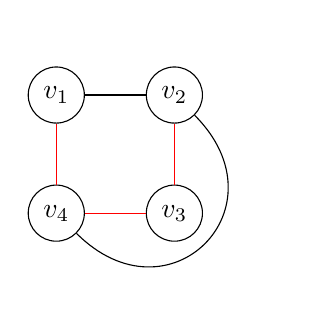
\begin{tikzpicture}[node distance={15mm}, main/.style = {draw, circle}] 
        \node[main] (1) {$v_1$}; 
        \node[main] (2) [right of=1] {$v_2$};
        \node[main] (3) [below of=2] {$v_3$}; 
        \node[main] (4) [left of=3] {$v_4$};

        \draw (1) -- (2);
        \draw [draw=red] (1) -- (4);
        \draw [draw=red] (2) -- (3);
        \draw (2) to [out=315, in=315, looseness=2] (4);
        \draw [draw=red] (3) -- (4);
    \end{tikzpicture} 
\end{center}
\vspace{-0.5cm}

The lines in red form a $v_1, v_2$-path, namely $v_1, v_4, v_3, v_2$. 
Another $v_1, v_2$-path can be obtained by simply traversing the edge $v_1v_2$. 

A {\bf cycle} in $G$ is a sequence of vertices $w_1, \dots, w_{k+1}$ 
such that $w_i w_{i+1} \in E$ for all $i = 1, \dots, k$, the vertices 
$w_1, \dots, w_k$ are all distinct, and $w_1 = w_{k+1}$.

Finally, a graph $G$ is {\bf connected} if for any pair of distinct vertices 
$u, v \in V$, there exists a $u, v$-path in $G$. 

\subsection{Shortest Paths Problem}\label{subsec:1.2}
Given a \emph{directed} graph $G = (V, E)$ with edge lengths $\ell_e \geq 0$
for each $e \in E$ and a distinguished start vertex $s \in V$, we wish 
to find shortest paths from $s$ to every other vertex in $V$. Note that 
when we work with directed graphs, we will denote the directed edges 
with $(v_1, v_2)$ as opposed to $v_1 v_2$ in the case of undirected graphs, where 
the order of the vertices did not matter. 

The {\bf length} of a path $P$ given by the sequence $w_1, \dots, w_k$ 
is given by 
\[ \ell(P) := \sum_{i=1}^{k-1} \ell_{(w_i, w_{i+1})} = \sum_{e\in P} \ell_e, \] 
where the second sum makes sense because there are no parallel edges. 
Then the {\bf shortest-path distance} from $s$ to a vertex $u \in V$ is 
defined to be
\[ d(u) := \min_{\text{$s,u$-paths $P$}} \ell(P). \] 
For example, we can consider the following instance of an undirected graph 
with given edge lengths and starting vertex $s = v_1$. 

\begin{center}
    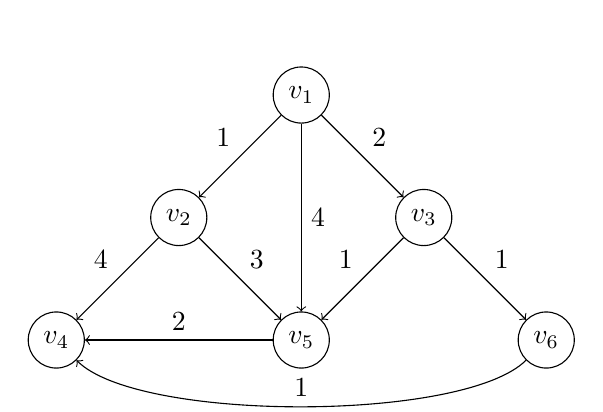
\begin{tikzpicture}[node distance={22mm}, main/.style = {draw, circle}] 
        \node[main] (1) {$v_1$}; 
        \node[main] (2) [below left of=1] {$v_2$};
        \node[main] (3) [below right of=1] {$v_3$}; 
        \node[main] (4) [below left of=2] {$v_4$};
        \node[main] (5) [below left of=3] {$v_5$};
        \node[main] (6) [below right of=3] {$v_6$};

        \draw[->] (1) -- node[midway, above left] {1} (2);
        \draw[->] (1) -- node[midway, above right] {2} (3);
        \draw[->] (1) -- node[midway, right] {4} (5);
        \draw[->] (2) -- node[midway, above left] {4} (4);
        \draw[->] (2) -- node[midway, above right] {3} (5);
        \draw[->] (3) -- node[midway, above left] {1} (5);
        \draw[->] (3) -- node[midway, above right] {1} (6);
        \draw[->] (5) -- node[midway, above] {2} (4);
        \draw[->] (6) to [out=225, in=315, looseness=0.5] node[midway, above] {1} (4);
    \end{tikzpicture} 
\end{center}
\vspace{-0.5cm}
In this case, we have $d(v_2) = 1$, since the only possible path from 
$v_1$ to $v_2$ is by taking the edge $(v_1, v_2)$. There are multiple
paths from $v_1$ to $v_5$; the shortest one is $v_1, v_3, v_5$ giving 
$d(v_5) = 3$. 

Note that we always set $d(s) = 0$. We now make some observations: 
\begin{enumerate}[(i)]
    \item If $(u, v) \in E$, then $d(v) \leq d(u) + \ell_{(u,v)}$, since 
    such an $s, v$-path is always an option.
    \item For every $v \in V$ distinct from $s$, there exists $w \in V$ 
    such that $d(v) = d(w) + \ell_{(w, v)}$ and $(w, v) \in E$. This can 
    be seen by chopping off the last edge from a shortest path from $s$ to $v$.
\end{enumerate}

\subsection{Dijkstra's Algorithm}\label{subsec:1.3}
In 1959, Dijkstra came up with the following algorithm to solve the 
shortest paths problem. The main idea is to maintain a set $A \subseteq V$ 
of ``explored'' nodes; that is, a set of nodes for which we already know the 
shortest-path distances. We'll also maintain labels $d'(v)$ for $v \in 
V \setminus A$ with upper bounds on the shortest-path distances from $s$. 

\begin{mdframed}[
    linewidth=1pt,
    linecolor=black,
    bottomline=false,topline=false,rightline=false,
    innerrightmargin=0pt,innertopmargin=0pt,innerbottommargin=0pt,
    innerleftmargin=1em,% Distance between vertical rule & proof content
    skipabove=0.75\baselineskip
]
{\bf Input.} A directed graph $G = (V, E)$, edge lengths $\ell_e \geq 0$ for 
all $e \in E$, and a start vertex $v \in V$. 

{\bf Output.} For all $v \in V$, the length $d(v)$ for the shortest-path from 
$s$ to $v$.
\begin{enumerate}[leftmargin=1.75cm, label={Step \arabic*.}]
    \item {\bf (Initialization.)} Set $A \gets \{s\}$, $d(s) \gets 0$, and $d'(v) \gets \infty$ 
    for all $v \in V \setminus A$.

    \item While $A \neq V$:
    \begin{enumerate}[label={Step 2.\arabic*.}]
        \item {\bf (Push down the upper bounds.)} For each $v \in V \setminus A$, compute 
        \[ d'(v) \gets \min\left\{ d'(v), \min_{\substack{u\in A \\ (u, v) \in E}} 
        \{ d(u) + \ell_{(u, v)} \} \right\}. \] 
        \item {\bf (Add a new vertex.)} Set $w \gets \argmin_{v \in V \setminus A} d'(v)$, 
        $A \gets A \cup \{w\}$, and $d(w) \gets d'(w)$. 
    \end{enumerate}
\end{enumerate}
\end{mdframed}\vspace{-0.25cm}

Suppose that for each vertex $w \in V$, we keep track of the node $u$ 
determining its upper bound $d'(w)$. That is, the node $u$ is such that 
$(u, w) \in E$ and $d'(w) = d(u) + \ell_{(u, w)}$. Then at the end of the 
algorithm, a shortest path from $s$ to $w$ can be obtained as a shortest path 
from $s$ to $u$ adjoined with the edge $(u, w) \in E$. Moreover, these edges 
selected by Dijkstra's algorithm form an arborescence, which is a nice graph 
structure that we'll discuss more later. 

Next, let's prove the correctness of Dijkstra's algorithm. In particular, 
we need to show that for every $v \in V$, the distance from $s$ to $v$ 
is computed correctly. We'll assume that the graph is connected; that is, 
for every $v \in V$, there is an $s, v$-path in $G$. (Note that the 
algorithm won't terminate otherwise, but it can be adjusted to deal 
with this.)

\begin{pf}[correctness of Dijkstra's algorithm]
    We proceed by induction on $|A|$, and show that at each point in time, 
    $d(v)$ is computed correctly for all $v \in A$. The case where $|A| = 1$ 
    is clear because at the start of the algorithm, we initialize $A = \{s\}$ 
    with $d(s) = 0$, which is correct. 

    Assume that $d(v)$ is computed correctly for every $v \in A$ when 
    that $|A| = k$. Suppose that we are adding a new vertex $w$ to $A$ 
    in Step 2.2 of the algorithm. Consider the vertex $u \in A$ such that 
    $(u, w) \in E$ and 
    \[ d'(w) = d(u) + \ell_{(u, w)}. \] 
    Specifically, this is the vertex $u$ determining the upper bound 
    $d'(w)$ which we discussed in the paragraph following the description 
    of the algorithm. 

    For the sake of contradiction, assume that the distance from $s$ to $w$ 
    is not $d'(w)$. Let $P_u$ be a shortest path from $s$ to $u$, and 
    let $P'$ be a shortest path from $s$ to $w$. Then by our 
    assumption, we know that 
    \[ \ell(P') < \ell(P_u) + \ell_{(u, w)} = d'(w). \] 
    Now, let $x, y \in V$ be such that $(x, y) \in E$ lies on the shortest 
    path $P'$ from $s$ to $w$, with $x \in A$ and $y \in V \setminus A$. 
    (This exists because at some point, the path must exit $A$ to get 
    from $s$ to $w$.) Then we obtain 
    \[ d'(y) \leq d(x) + \ell_{(x,y)} \leq \ell(P') < \ell(P_u) 
    + \ell_{(u, w)} = d'(w), \] 
    where the first inequality is because of how $d'(y)$ is computed in 
    Step 2.1, and the second inequality is because the shortest path 
    from $x$ to $y$ adjoined with the edge $(x, y)$ is part of the path $P'$, 
    noting that $\ell_e \geq 0$ for all $e \in E$. But this contradicts 
    our choice of $w = \argmin_{v\in V \setminus A} \{d'(v)\}$ in Step 2.2 
    since $y \in V \setminus A$ but $d'(y) < d'(w)$. \qed
\end{pf}\vspace{-0.25cm}

The {\bf running time} of an algorithm is the number of elementary operations 
that the algorithm performs as a function of the input size. The {\bf input 
size} is the number of bits needed to specify the input. 
\begin{itemize}
    \item For example, in order to specify an integer $n \geq 0$ in binary, 
    we require about $\log_2(n)$ bits. 
    \item To specify a graph $G = (V, E)$ with integral edge lengths 
    $\ell_e \geq 0$ for each $e \in E$, we require approximately 
    $|V| + |E| + \sum_{e\in E} \log_2(\ell_e)$ bits. Note that we can 
    specify an edge with two pointers to the endpoints.
\end{itemize} 
We will need big-$O$ notation to describe running time, because we are 
interested in the asymptotic behaviour of algorithms. For two functions
$f : \R^+ \to \R^+$ and $g : \R^+ \to \R^+$, we say that $f(n) = 
O(g(n))$ if there exist constants $n_0 \in \N$ and $c \geq 0$ such that 
$f(n) \leq c \cdot g(n)$ for all $n \geq n_0$. For example, we have 
$2n^2 + 1 = O(n^2)$ and $\log(n) = O(n)$. An algorithm is then considered 
{\bf efficient} if its running time is bounded above by a polynomial function 
of the input size. 

Let's consider the running time of Dijkstra's algorithm by looking 
at a naive implementation. For ease of notation, we will write 
$|V| = n$ and $|E| = m$. Note that $G = (V, E)$ is connected, 
so $n-1 \leq m \leq n^2$.
\begin{itemize}
    \item Step 1 can be performed using $O(n)$ operations since we are only
    assigning values for each vertex. 
    \item In Step 2, there are at most $n$ iterations. 
    \begin{itemize}
        \item Step 2.1 can be performed using $O(m)$ operations because 
        each edge will participate in at most two comparisons throughout the 
        entire iteration. 
        \item Step 2.2 takes $O(n)$ operations in order to determine the 
        vertex of minimum upper bound. 
    \end{itemize}
\end{itemize}
Therefore, the running time of the naive implementation is 
$O(n + mn + n^2) = O(mn)$, which is polynomial in the input size.  

We note that there are better implementations of Dijkstra's algorithm 
than the naive one that we have just stated. For Step 2.1, we can 
use $m$ \textsc{Decrease-Key} calls and for Step 2.2, we can use 
$n$ \textsc{Extract-Min} calls. In particular, by using Fibonacci heaps, 
\textsc{Decrease-Key} has running time $O(1)$ and \textsc{Extract-Min} 
has running time $O(\log n)$, which brings the total running time down to 
$O(m + n\log n)$.\newpage
\section{Minimum Spanning Trees}\label{sec:2}

\subsection{Trees}\label{subsec:2.1}
A {\bf tree} is a connected acyclic graph; that is, a connected graph 
containing no cycles. 
\begin{center}
    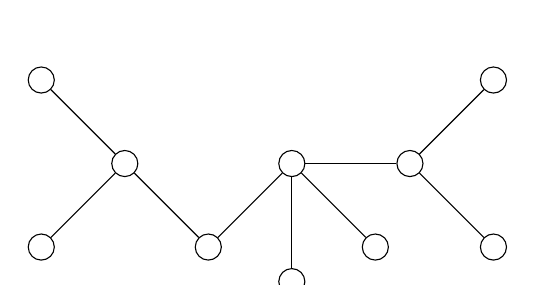
\begin{tikzpicture}[node distance={15mm}, main/.style = {draw, circle}] 
        \node[main] (1) {}; 
        \node[main] (2) [below right of=1] {};
        \node[main] (3) [below left of=2] {}; 
        \node[main] (4) [below right of=2] {};
        \node[main] (5) [above right of=4] {};
        \node[main] (6) [below of=5] {};
        \node[main] (7) [below right of=5] {};
        \node[main] (8) [right of=5] {};
        \node[main] (9) [above right of=8] {};
        \node[main] (10) [below right of=8] {};

        \draw (1) -- (2); \draw (2) -- (3); \draw (2) -- (4);
        \draw (4) -- (5); \draw (5) -- (6); \draw (5) -- (7);
        \draw (5) -- (8); \draw (8) -- (9); \draw (8) -- (10);
    \end{tikzpicture} 
\end{center}
\vspace{-0.25cm}
Given a graph $G = (V, E)$, a {\bf spanning tree} of $G$ is a graph $T = (V, F)$ 
such that $F \subseteq E$ and $T$ is a tree. We illustrate an example of a 
graph $G$ with a subtree $T$ using bold edges below. 
\begin{center}
    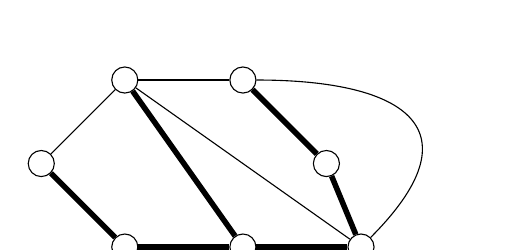
\begin{tikzpicture}[node distance={15mm}, main/.style = {draw, circle}] 
        \node[main] (1) {}; 
        \node[main] (2) [right of=1] {};
        \node[main] (3) [below left of=1] {}; 
        \node[main] (4) [below right of=2] {};
        \node[main] (5) [below right of=3] {};
        \node[main] (6) [right of=5] {};
        \node[main] (7) [right of=6] {};

        \draw (1) -- (2); 
        \draw (1) -- (3); 
        \draw [line width=2pt] (1) -- (6);
        \draw (1) -- (7);
        \draw [line width=2pt] (2) -- (4);
        \draw (2) to [out=0, in=45, looseness=2] (7);
        \draw [line width=2pt] (3) -- (5);
        \draw [line width=2pt] (4) -- (7);
        \draw [line width=2pt] (5) -- (6);
        \draw [line width=2pt] (6) -- (7);
    \end{tikzpicture} 
\end{center}
In an introductory graph theory course, such as MATH 239, 
it is shown that every tree on $n$ vertices has $n-1$ edges. The following 
theorem then gives us a useful characterization of trees. 

\begin{theo}[Fundamental Theorem of Trees]{theo:2.1}
    Let $T = (V, F)$ be a graph. The following are equivalent:
    \begin{enumerate}[(i)]
        \item $T$ is a tree. 
        \item $T$ is connected and $|F| = |V| - 1$. 
        \item $T$ is acyclic and $|F| = |V| - 1$. 
    \end{enumerate}
\end{theo}

In particular, if we know that two of the conditions hold, then the 
third one is guaranteed.

\subsection{Minimum Spanning Trees}\label{subsec:2.2}
Given a connected graph $G = (V, E)$ and edge costs $c_e$ for each 
$e \in E$, our goal is to find a spanning tree $T$ of minimum cost 
\[ c(T) := \sum_{e \in T} c_e. \] 
First, we'll set some notation. For a vertex $v \in V$, we define 
$\delta(v)$ to be the set of edges in $E$ incident to $v$. More generally, 
given a subset of vertices $S \subseteq V$, the {\bf cut induced by $S$} is 
defined to be the set 
\[ \delta(S) := \{uv \in E : u \in S,\, v \notin S\}. \] 
The following theorem will be extremely important for finding a minimum 
spanning tree. 

\begin{theo}[Cut Property]{theo:2.2}
    Suppose that the costs $c_e$ for $e \in E$ are distinct. 
    Let $S \subseteq V$ be such that $S \neq \varnothing$ and $S \neq V$, 
    and let 
    \[ e = \argmin_{f \in \delta(S)} c_f. \] 
    Then every minimum spanning tree contains the edge $e$. 
\end{theo}
\begin{pf}[Theorem~\ref{theo:2.2}]
    We proceed by contradiction. Let $S \subseteq V$ be such that $S 
    \neq \varnothing$ and $S \neq V$, and let $e = \argmin_{f\in S} c_f$. 
    Suppose that there is a minimum spanning tree $T = (V, F)$ such that 
    $e \notin F$. 

    Consider the graph $(V, F \cup \{e\})$. Note that $|F \cup \{e\}| = |V|$ 
    and this graph is connected, so it cannot be a tree by Theorem~\ref{theo:2.1}. 
    In particular, it must contain a cycle $C$. 

    Next, note that $|C \cap \delta(S)|$ must be even because for any 
    edge leaving the cut $\delta(S)$, there must be another edge coming back 
    into the cut. Moreover, since $e \in C \cap \delta(S)$, we have 
    $C \cap \delta(S) \neq \varnothing$. This implies that 
    $|C \cap \delta(S)| \geq 2$, so there is another edge $e' \neq e$ 
    with $e' \in C \cap \delta(S)$.

    Consider now the graph $T' = (V, (F \cup \{e\}) \setminus \{e'\})$. 
    Then $|(F \cup \{e\}) \setminus \{e'\}| = |F| = |V| - 1$ and $T'$ is 
    connected because if a path between two vertices used the edge $e'$, 
    then we could go along the edges in $C \setminus \{e'\}$ instead. 
    So by Theorem~\ref{theo:2.1}, $T'$ is also a spanning tree. 
    Finally, observe that 
    \[ c(T) - c(T') = c_{e'} - c_e > 0 \] 
    because we have $e = \argmin_{f\in S} c_f$ and $e' \neq e$ with 
    $e' \in \delta(S)$, as well as the assumption that the edge 
    costs $c_e$ for $e \in E$ were distinct. But $T'$ has lower cost 
    than $T$, contradicting our assumption that $T$ was a minimum 
    spanning tree. \qed
\end{pf}\vspace{-0.25cm}

The following property relating cycles to minimum spanning trees 
can also be proved similarly to Theorem~\ref{theo:2.2}. 
The main idea is to try to create shortcuts using the edges in the cycle. 

\begin{theo}[Cycle Property]{theo:2.3}
    Let $G = (V, E)$ be connected with distinct edge costs 
    $c_e$ for $e \in E$. Let $C$ be a cycle in $G$ and let 
    \[ e = \argmax_{f\in C} c_f. \] 
    Then no minimum spanning tree contains the edge $e$. 
\end{theo}

\subsection{Prim's Algorithm}\label{subsec:2.3}
Prim's algorithm takes the idea of the cut property (Theorem~\ref{theo:2.2}) 
and uses it to compute a minimum spanning tree starting from an arbitrary 
vertex $s \in V$. At each iteration of the algorithm, we will keep track of a 
set of a partial tree construction $T$ and vertices $A \subseteq V$ that are 
connected to $s$ in $T$. 

\begin{mdframed}[
    linewidth=1pt,
    linecolor=black,
    bottomline=false,topline=false,rightline=false,
    innerrightmargin=0pt,innertopmargin=0pt,innerbottommargin=0pt,
    innerleftmargin=1em,% Distance between vertical rule & proof content
    skipabove=0.75\baselineskip
]
{\bf Input.} A graph $G = (V, E)$ and edge costs $c_e$ for 
all $e \in E$. 

{\bf Output.} A minimum spanning tree of $G$.
\begin{enumerate}[leftmargin=1.75cm, label={Step \arabic*.}]
    \item {\bf Initialization.} Let $s \in V$ be an arbitrary vertex, 
    then set $A \gets \{s\}$ and $T \gets \varnothing$.

    \item While $A \neq V$:
    \begin{enumerate}[label={Step 2.\arabic*.}]
        \item {\bf Pick an edge for the minimum spanning tree.} 
        Set 
        \[ e \gets \argmin_{f \in \delta(A)} c_f, \] 
        where $e = uv$ with $u \in A$ and $v \notin A$.  
        \item {\bf Update values.} Set $A \gets A \cup \{v\}$ and 
        $T \gets T \cup \{e\}$. 
    \end{enumerate}
\end{enumerate}
\end{mdframed}\vspace{-0.15cm}

Let's run Prim's algorithm on a simple example. Consider the following 
graph $G = (V, E)$, and suppose that at Step 1, we pick $v_1$ to be 
the initial vertex. 
\begin{center}
    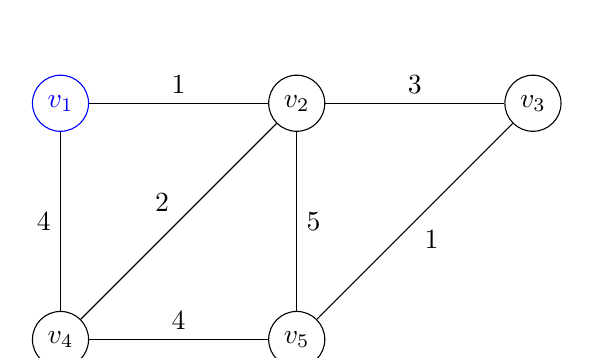
\begin{tikzpicture}[node distance={30mm}, main/.style = {draw, circle}] 
        \node[main, color=blue] (1) {$v_1$}; 
        \node[main] (2) [right of=1] {$v_2$};
        \node[main] (3) [right of=2] {$v_3$}; 
        \node[main] (4) [below of=1] {$v_4$};
        \node[main] (5) [right of=4] {$v_5$};

        \draw (1) -- node[midway, above] {1} (2);
        \draw (2) -- node[midway, above] {3} (3);
        \draw (1) -- node[midway, left] {4} (4);
        \draw (2) -- node[midway, above left] {2} (4);
        \draw (2) -- node[midway, right] {5} (5);
        \draw (3) -- node[midway, below right] {1} (5);
        \draw (5) -- node[midway, above] {4} (4);
    \end{tikzpicture} 
\end{center}
\vspace{-0.25cm}
Then at the first iteration of Step 2.1, we have $\delta(A) = 
\{v_1v_2, v_1v_4\}$, so we pick $e = v_1v_2$ because it has minimum cost.
At Step 2.2, we set $A = \{v_1, v_2\}$ and $T = \{v_1v_2\}$. 

\begin{center}
    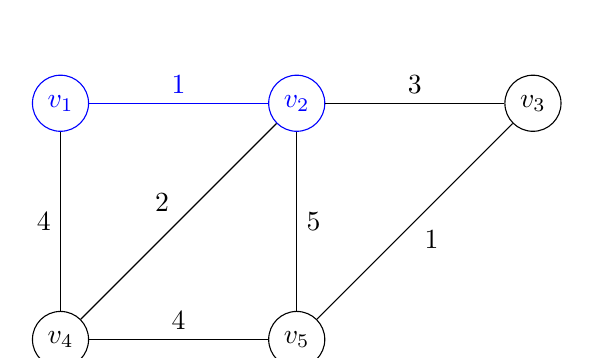
\begin{tikzpicture}[node distance={30mm}, main/.style = {draw, circle}] 
        \node[main, color=blue] (1) {$v_1$}; 
        \node[main, color=blue] (2) [right of=1] {$v_2$};
        \node[main] (3) [right of=2] {$v_3$}; 
        \node[main] (4) [below of=1] {$v_4$};
        \node[main] (5) [right of=4] {$v_5$};

        \draw[color=blue] (1) -- node[midway, above] {1} (2);
        \draw (2) -- node[midway, above] {3} (3);
        \draw (1) -- node[midway, left] {4} (4);
        \draw (2) -- node[midway, above left] {2} (4);
        \draw (2) -- node[midway, right] {5} (5);
        \draw (3) -- node[midway, below right] {1} (5);
        \draw (5) -- node[midway, above] {4} (4);
    \end{tikzpicture} 
\end{center}
\vspace{-0.25cm}
The edge $v_2v_4$ is of minimum cost in the cut induced by $A$, so 
we set $A = \{v_1, v_2, v_4\}$ and $T = \{v_1v_2, v_2v_4\}$ at the next iteration. 
Continuing in this fashion, we obtain the following minimum spanning tree.

\begin{center}
    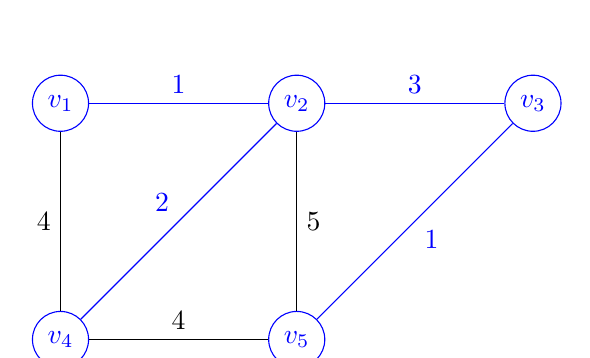
\begin{tikzpicture}[node distance={30mm}, main/.style = {draw, circle}] 
        \node[main, color=blue] (1) {$v_1$}; 
        \node[main, color=blue] (2) [right of=1] {$v_2$};
        \node[main, color=blue] (3) [right of=2] {$v_3$}; 
        \node[main, color=blue] (4) [below of=1] {$v_4$};
        \node[main, color=blue] (5) [right of=4] {$v_5$};

        \draw[color=blue] (1) -- node[midway, above] {1} (2);
        \draw[color=blue] (2) -- node[midway, above] {3} (3);
        \draw (1) -- node[midway, left] {4} (4);
        \draw[color=blue] (2) -- node[midway, above left] {2} (4);
        \draw (2) -- node[midway, right] {5} (5);
        \draw[color=blue] (3) -- node[midway, below right] {1} (5);
        \draw (5) -- node[midway, above] {4} (4);
    \end{tikzpicture} 
\end{center}
\vspace{-0.25cm}
Note that Prim's algorithm may seen similar to Dijkstra's algorithm 
which also yields a spanning tree in the process of computing shortest paths. 
However, these algorithms fundamentally solve different problems, and 
there are examples where the resulting spanning trees do not coincide. 
Moreover, Dijkstra's algorithm takes a directed graph as input, 
whereas Prim's algorithm takes an undirected graph. 

Next, let's prove that Prim's algorithm always gives us a minimum spanning tree. 
For simplicity, we will assume that all edge costs $c_e$ for 
$e \in E$ are distinct. 

\begin{pf}[correctness of Prim's algorithm]
    At every iteration of Step 2, we add one edge to $T$, and we run 
    through $|V| - 1$ iterations. Therefore, $T$ has exactly 
    $|V| - 1$ edges. Moreover, an invariant of Prim's algorithm is that 
    all vertices in $A$ remain connected to $s$, so the final output is 
    also connected. Therefore, we indeed obtain a spanning tree by 
    Theorem~\ref{theo:2.1}. Finally, by the cut property (Theorem~\ref{theo:2.2})
    and our assumption that all the edge costs are distinct, $T$ contains 
    only the edges that are in every minimum spanning tree, so $T$ 
    itself is a minimum spanning tree. \qed 
\end{pf}

As a consequence, we also have the following useful result. 

\begin{cor}{cor:2.4}
    Let $G = (V, E)$ be a connected graph with distinct edge costs $c_e$ for 
    $e \in E$. Then $G$ has a unique minimum spanning tree.
\end{cor}

As usual, let's consider the running time, denoting $|V| = n$ 
and $|E| = m$. For an efficient implementation, 
we keep track of a key $d'(v)$ for each $v \in V \setminus A$. 
Once a vertex $w$ is added to $A$ in Step 2.2, we update the keys via 
$d'(v) \gets \min\{d'(v), c_{wv}\}$ for each $v \in V \setminus A$. 

Note that Step 1 takes $O(1)$ time, and 
there are $n-1$ iterations of Step 2. Implementing Prim's algorithm 
using priority queues, we note that each iteration of Step 2.1 
involves one \textsc{Extract-Min} call, and 
going through all iterations of Step 2.2 takes at most $m$ 
\textsc{Decrease-Key} calls in total. We recall that by using Fibonacci heaps, 
\textsc{Decrease-Key} is $O(1)$ and \textsc{Extract-Min} is $O(\log n)$, 
so we have a total running time of $O(n\log n + m)$. \newpage

\end{document}
